


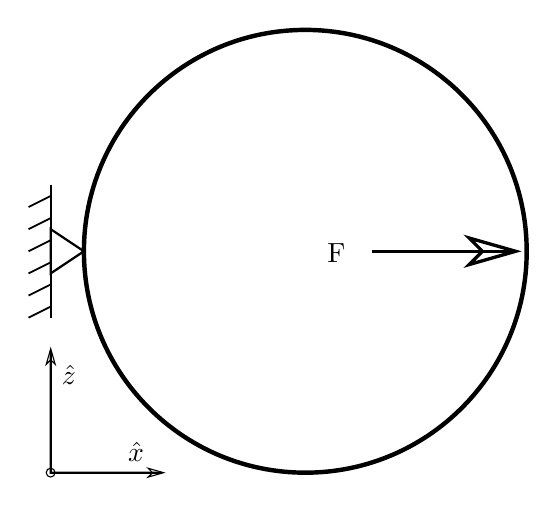
\begin{tikzpicture}[y=0.80pt, x=0.8pt,yscale=-1, inner sep=0pt, outer sep=0pt]
\begin{scope}[shift={(0,-552.36218)}]
  \path[shift={(0,552.36218)},draw=black,fill=black,line join=round,miter
    limit=4.00,fill opacity=0.000,nonzero rule,line width=1.600pt]
    (350.0000,250.0000) .. controls (350.0000,305.2285) and (305.2285,350.0000) ..
    (250.0000,350.0000) .. controls (194.7715,350.0000) and (150.0000,305.2285) ..
    (150.0000,250.0000) .. controls (150.0000,194.7715) and (194.7715,150.0000) ..
    (250.0000,150.0000) .. controls (305.2285,150.0000) and (350.0000,194.7715) ..
    (350.0000,250.0000) -- cycle;
    \path[color=black,fill=black,line width=1.200pt] (280.0000,801.6122) --
      (280.0000,803.1122) -- (345.0000,803.1122) -- (345.0000,801.6122) --
      (280.0000,801.6122) -- cycle;
    \path[draw=black,even odd rule,line width=1.200pt] (330.0000,802.3622) --
      (324.0000,808.3622) -- (345.0000,802.3622) -- (324.0000,796.3622) --
      (330.0000,802.3622) -- cycle;
  \path[shift={(0,552.36218)},draw=black,line join=miter,line cap=butt,line
    width=0.800pt] (135.0000,240.0000) -- (150.0000,250.0000) --
    (135.0000,260.0000) -- cycle;
  \path[draw=black,line join=miter,line cap=butt,miter limit=4.00,line
    width=0.640pt] (135.0000,787.3622) -- (125.0000,792.3622);
  \path[draw=black,line join=miter,line cap=butt,miter limit=4.00,line
    width=0.640pt] (135.0000,807.3622) -- (125.0000,812.3622);
  \path[draw=black,line join=miter,line cap=butt,miter limit=4.00,line
    width=0.640pt] (135.0000,817.3622) -- (125.0000,822.3622);
  \path[draw=black,line join=miter,line cap=butt,miter limit=4.00,line
    width=0.640pt] (135.0000,797.3622) -- (125.0000,802.3622);
  \path[draw=black,line join=miter,line cap=butt,miter limit=4.00,line
    width=0.640pt] (135.0000,827.3622) -- (125.0000,832.3622);
  \path[shift={(0,552.36218)},draw=black,line join=miter,line cap=butt,line
    width=0.800pt] (135.0000,220.0000) -- (135.0000,280.0000);
  \path[draw=black,line join=miter,line cap=butt,miter limit=4.00,line
    width=0.640pt] (135.0000,777.3622) -- (125.0000,782.3622);
  \path[fill=black] (260,807.36218) node[above right] (text4591) {F};
    \path[color=black,fill=black,line width=0.800pt] (134.5000,847.3622) --
      (134.5000,902.3622) -- (134.5000,902.8622) -- (135.0000,902.8622) --
      (185.0000,902.8622) -- (185.0000,901.8622) -- (135.5000,901.8622) --
      (135.5000,847.3622) -- (134.5000,847.3622) -- cycle;
    \path[draw=black,even odd rule,line width=0.400pt] (135.0000,851.3622) --
      (137.0000,853.3622) -- (135.0000,846.3622) -- (133.0000,853.3622) --
      (135.0000,851.3622) -- cycle;
    \path[draw=black,even odd rule,line width=0.400pt] (136.3859,903.7481) ..
      controls (135.6053,904.5288) and (134.3382,904.5288) .. (133.5575,903.7481) ..
      controls (132.7769,902.9675) and (132.7769,901.7003) .. (133.5575,900.9197) ..
      controls (134.3382,900.1390) and (135.6053,900.1390) .. (136.3859,900.9197) ..
      controls (137.1666,901.7003) and (137.1666,902.9675) .. (136.3859,903.7481) --
      cycle;
    \path[draw=black,even odd rule,line width=0.400pt] (181.0000,902.3622) --
      (179.0000,904.3622) -- (186.0000,902.3622) -- (179.0000,900.3622) --
      (181.0000,902.3622) -- cycle;
  \path[shift={(0,552.36218)},fill=black] (140,310.35715) node[above right]
    (text5495) {$\hat{z}$};
  \path[fill=black] (170,897.36218) node[above right] (text5499) {$\hat{x}$};
\end{scope}

\end{tikzpicture}

